\documentclass{article}
\date{}
\title{Assignment No. 1}
\usepackage{graphicx}

\begin{document}
	
	\maketitle
	
	\section{Title:}
	Using Divide and Conquer Strategies design a function for Binary Search using C++/Java/Python/Scala.
	
	
	\section{Theory:}
	
	\subsection{Divide and Conquer:}
	
	\begin{itemize}
		
		\item Given a function to compute on an inputs the divide and conquer strategy suggest splitting the input into k distinct input sets ,such that 1<k<n yielding k sub problems.\\
		\item These sub problems must be solve and then method must be found to combine the sub solution into a solution of a whole.\\
		\item If the sub problems are relatively large then the divide and conquer strategy can be possibly reapplied.\\
		\item Often the sub problems are of the same type as the same original problem for which the reapplication of divide and conquer principle is naturally expressed by a recursive algorithm.\\
		
	\end{itemize}
	
	\subsection{Binary Search:}
	
	\begin{itemize}
		
		\item Binary search can be implemented using a binary decision tree.\\
		\item Example:Consider the following-\\
		Sorted array: L = [1, 3, 4, 6, 8, 9, 11] \\
		Target value: X = 4\\
		Compare X to 6. X is smaller. Repeat with L = [1, 3, 4].\\
		Compare X to 3. X is larger. Repeat with L = [4].\\
		Compare X to 4. X equals 4, so the position is returned.\\
		
	\end{itemize}
	
	\subsection{Applying divide and conquer approach on binary search tree:}
	
	\begin{itemize}
		
		\item If divide and conquer approach is use for generating the binary search tree, the input element set is to be divided into subset such that BST can be generated for each subset.\\
		\item The problem occurs when these BST's are generated from the subset are to be merged into a single BST consisting of all the input elements.\\
		\item Consider the following \\
		Let the input set\\ 
		I={7,6,5,8,13,2,14,9}\\
		If we divide the input set into two parts then \\
		I1={7,6,5,8} I2={13,2,14,9}\\
		then respective BST's are \\
	\end{itemize}
	
	\begin{figure}[h!]
		\centering
		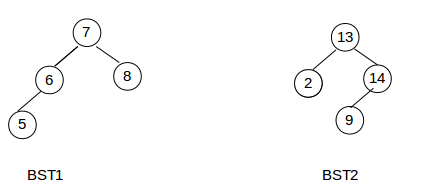
\includegraphics[scale=0.7]{q.png}
	\end{figure}
	\begin{figure}[h!]
		\centering
		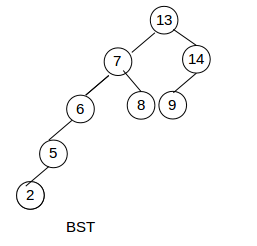
\includegraphics[scale=0.7]{p.png}
	\end{figure}
	
	\subsection{Proposal :}
	\begin{itemize}
		\item In the proposed approach we divide the input into two parts such that all the elements smaller than the first element are in the first sub part and all those greater than the first element are in the second sub part.\\
		I={7,6,5,8,13,2,14,9}\\
		
		I1={7,6,5,2} I2={7,8,13,14,9}\\
		Also preserving the order in which they appear in I1.\\
		BST's thus formed from I1 and I2 will be now as follow\\
		\begin{figure}[h!]
			\centering
			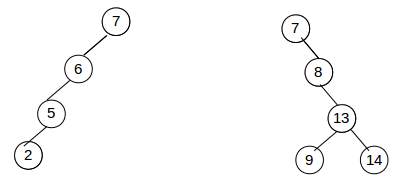
\includegraphics[scale=0.7]{r.png}
		\end{figure}
		
		\item Now we can easily merge the two BSTs as follow\\
		\begin{figure}[h!]
			\centering
			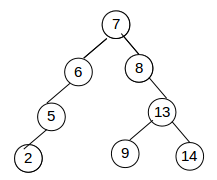
\includegraphics[scale=0.7]{s.png}
		\end{figure}
		
	\end{itemize}
	\section{Mathematical model:}
	\begin{itemize}
		
		\item Input–a. Elements in ascending order\\
		b. Element to be searched\\
		\item Output – Element location\\
		\item Formula – :a. Mid= lower+upper/2\\
		b. a[mid+1]\\
		\item Algorithm-\\
		1. Start\\
		2. Binary-search (A, first, last)\\
		3. if first > last // (i.e., nothing to search)\\
		4. return false\\
		5. otherwise\\
		6. middle <=(first+ last)\\
		7. if A[middle]matches key\\
		8. return true.\\
		9. otherwise.\\
		10. if A[middle]> key.\\
		11. return.\\
		12. Bin-search(A, first,middle -1, key).\\
		13. otherwise.\\
		14. return\\
		15. Bin-search(A, middle +1, last, key).\\
		16. Post: returns true if key is in A [first...last].\\
		17. Stop\\
	\end{itemize}         
	\section{Testing:}
	\subsection{Blackbox Testing:}
	\begin{itemize}
		\item Black-box testing is a method of software testing that examines the\\ function- ability of an application without peering into its internal\\ structures or workings.\\
		\item This method of test can be applied to virtually every level of\\ software testing:unit, integration, system and acceptance\\
		\item Input:Sorted array of N elements, Key to be searched\\
		\item output:Position of key after searching
		Example shown in the above table\\
	\end{itemize}
	
	\begin{figure}[h!]
		\centering
		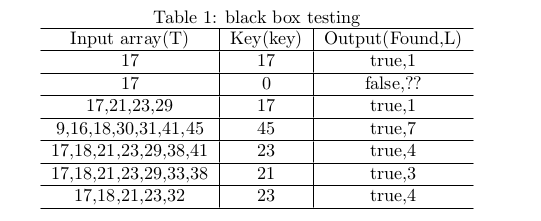
\includegraphics[scale=0.7]{table.png}
	\end{figure}
	
	\subsection{White Box Testing:}
	
	White-box testing (also known as clear box testing, glass box testing, transparent box testing, and structural testing) is a method of testing software that tests internal structures or workings of an application, as opposed to its functionality(i.e. black-box testing). While developing 
	test cases for white box testing it is understood that complete testing 
	is impossible. In White Box testing we checkup to which extent the code 
	is being executed, i.e. Covered. There are different kinds of coverage like, statement coverage, path coverage, etc. We will use one of the most popular technique i.e. Statement coverage. Statement coverage is a white box testing technique, which involves the execution of all the statements at least once in the source code. It is a metric, which is used to calculate and measure the number of statements in the source code which have been executed. For this, we will use Flow Graphs. Flow graphs are, Syntactic abstraction of source code Resembling to classical flow charts Forms the basis for white box test case generation principles.Conventions of flow graph notation, \\
	Sample Input: For integer array int A[] = 1,2,3,4,5,6,7,8,9,10; Function 
	is passed\\
	following arguments: Binary Search(A, 1, 10, 7);\\
	Output obtained: Entered second Entered third Entered first 6\\
	The underlined nodes are the ones being tested. The above output shows
	that every test region is covered for given input.\\
	\begin{figure}[h!]
		\centering
		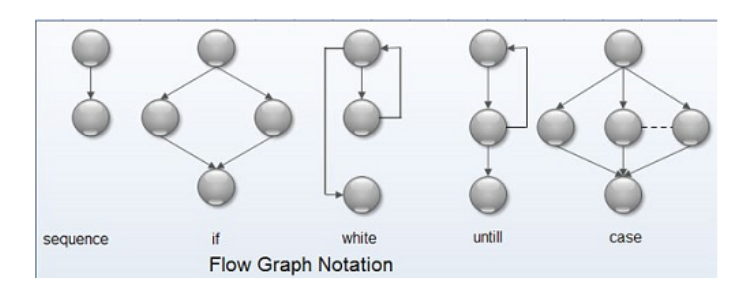
\includegraphics[scale=0.5]{pqr.png}
	\end{figure}
	
	\begin{figure}[h!]
		\centering
		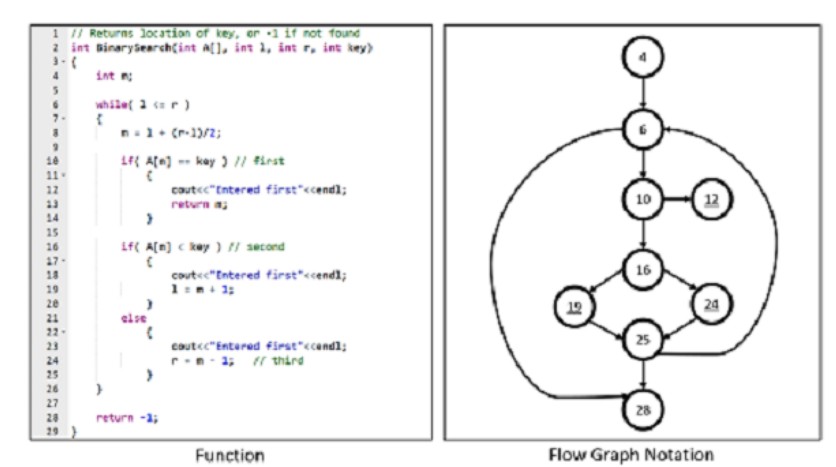
\includegraphics[scale=0.5]{xyz.png}
	\end{figure}
	
	\subsection{Positive/Negative Testing:}
	\begin{itemize}
		\item Position Testing :The element entered in ascending order then correct location of key will be found\\
		Example- Input sequence(17) key (17) output(true ,1)\\
		\item Negative Testing :The element not entered in ascending order then wrong location of key will be found\\
		Example- Input sequence(17) key (0) output(false,??)\\
	\end{itemize}
	
	\section{Conclusion:}
	From this experiment, we have successfully ,implemented binary search
	using divide and conquer strategies.
	
	\begin{center}
		\begin{tabular}
			{|c|c|c|c|c|}\hline
			{\bf Roll No.}		&{\bf Name of Student}	&{\bf Date of Performance}  				&{\bf Date of Submission}	&{\bf Sign.}  \\    \hline
			BECOC357	& Sunny Shah &  22 / 06 / 2017		& 29 / 06 / 2017		&  \\ \hline
		\end{tabular}\\ 
	\end{center}
	
\end{document}
